% Solutions to the five homework assignments. Written for this edition; the handouts contain no solutions.
% Every numerical value here was recomputed (see CORRECTIONS.md, "How the formulas were checked").
\section{Solutions to the homework problems}\label{sec:solutions}

The handouts give no solutions; these were written for this edition. They use the notation of the lectures, and each
one links back to its problem.

% ======================================================================
\subsection{Homework assignment 1}

\solution{1}{1}
\solpart{(a)} At $T = -13^\circ\text{C} = 260.15$~K and $p = 1$~atm $= 1.013\times 10^5$~Pa the ideal gas law gives the
number density
\begin{equation}
  \rho_n = \frac{p}{\kB T} = \frac{1.013\times 10^5\ \text{Pa}}{(1.381\times 10^{-23}\ \text{J/K})(260.15\ \text{K})}
  = 2.82\times 10^{25}\ \text{m}^{-3}.
\end{equation}
Each molecule has on average the volume $1/\rho_n$ to itself, so the mean distance between molecules is
\begin{equation}
  d\simeq\rho_n^{-1/3} = 3.3\times 10^{-9}\ \text{m} = 3.3\ \text{nm}.
\end{equation}

\solpart{(b)} The bond lengths are $0.110$~nm for N$_2$ and $0.121$~nm for O$_2$. Including the electron clouds, the
effective diameter of either molecule is about $\sigma\approx 0.35$~nm. So $d/\sigma\approx 10$: neighboring molecules
are about ten molecular diameters apart.

\solpart{(c)} The ideal gas law leaves out the volume of the molecules and the forces between them, and both
corrections are small when $\sigma\ll d$. The fraction of the volume excluded by the molecules is of order
$(\sigma/d)^3\sim 10^{-3}$. For a quantitative estimate, the van der Waals constants of N$_2$,
$a = 0.137$~Pa\,m$^6$/mol$^2$ and $b = 3.87\times 10^{-5}$~m$^3$/mol, give the second virial coefficient
$B_2 = b-a/(RT) = -2.5\times 10^{-5}$~m$^3$/mol at 260~K, and
\begin{equation}
  \frac{pV}{N\kB T}-1\simeq\frac{B_2\,p}{RT}\simeq -1.1\times 10^{-3}.
\end{equation}
At this temperature and pressure the ideal gas law holds to about 0.1\%.

\solution{1}{2}
\solpart{(a)} $M$ vanishes where the factor $1-6u+u^2$ does. Its roots are $u = 3\mp 2\sqrt2$. For $0<T<\infty$,
$u = e^{-4K}$ lies in $(0,1)$ and increases with $T$, so the transition is at
\begin{equation}
  u_c = 3-2\sqrt2 = (\sqrt2-1)^2 = 0.1716 ,
\end{equation}
and $1-6u+u^2>0$ for $u<u_c$, i.e.\ $T<T_c$, as it must be for $M$ to be real. Then $e^{-2K_c} = \sqrt2-1$, so
\begin{equation}
  K_c = \frac{1}{2}\ln(1+\sqrt2) = 0.4407,\qquad \kB T_c = \frac{J}{K_c} = \frac{2J}{\ln(1+\sqrt2)} = 2.269\,J ,
\end{equation}
the same as the critical temperature of the square-lattice Ising model.

\solpart{(b)} Write $1-6u+u^2 = (u_c-u)(u_+-u)$ with $u_+ = 3+2\sqrt2$. Near $T_c$,
$u_c-u\simeq(\dd u/\dd T)_c(T_c-T)$ with $\dd u/\dd T = 4Ju/(\kB T^2)>0$, while the factors $(1+u)^{1/4}$,
$(u_+-u)^{1/7}$ and $(1-u)^{-1/2}$ are smooth and nonzero. So $M\propto(u_c-u)^{1/7}\propto(T_c-T)^{1/7}$ and
\begin{equation}
  \beta = \frac{1}{7}.
\end{equation}

\solution{1}{3}
Set $T = T_c(1+\tau)$ with $\tau\to 0^+$. Then $(T/T_c)^8-1 = (1+\tau)^8-1 = 8\tau+\Order(\tau^2)$, so
\begin{equation}
  \chi_0\simeq\frac{b}{(8\tau)^{3/2}} = \frac{b}{16\sqrt2}\,\tau^{-3/2},
\end{equation}
and $\gamma = 3/2$.

\solution{1}{4}
For $J<0$, $K = -\beta|J|\to-\infty$ as $T\to 0$, so $e^{-4K} = e^{4\beta|J|}\to\infty$, and $|h| = \beta|H|\to\infty$.
For large $\beta$, $\sinh^2h\simeq e^{2\beta|H|}/4$ and
\begin{equation}
  M\simeq\sgn(H)\,\frac{e^{\beta|H|}/2}{\left[e^{2\beta|H|}/4+e^{4\beta|J|}\right]^{1/2}}.
\end{equation}
Which term in the denominator wins depends on how $|H|$ compares with $2|J|$. If $|H|<2|J|$, the second term
dominates and $M\simeq\sgn(H)\,e^{-\beta(2|J|-|H|)}/2\to 0$. If $|H|>2|J|$, the first term dominates and
$M\to\sgn(H)$. At $|H| = 2|J|$ both grow like $e^{4\beta|J|}$ and $M\to\sgn(H)(1/2)/(1/4+1)^{1/2}$. So at $T = 0$,
\begin{equation}
  M = \begin{cases} 0 & |H|<2|J|\\[2pt] \sgn(H)/\sqrt5 & |H| = 2|J|\\[2pt] \sgn(H) & |H|>2|J| .\end{cases}
\end{equation}
The antiferromagnetic coupling favors the N\'eel state $\cdots\uparrow\downarrow\uparrow\downarrow\cdots$, with energy
$-|J|$ per site and $M = 0$; the field favors the aligned state, with energy $|J|-|H|$ per site. The aligned state wins
when $|H|>2|J|$. At $|H| = 2|J|$, reversing an isolated spin of the aligned state lowers the bond energy by $4|J|$ and
raises the field energy by $2|H|$, so every configuration with no two adjacent reversed spins is a ground state. There
are about $\phi^N$ of them, with $\phi = (1+\sqrt5)/2$, and the fraction of reversed spins among them is
$(1-1/\sqrt5)/2$, which gives $M = 1/\sqrt5$ again. The ground state at this field has nonzero entropy, $\kB\ln\phi$
per site.

\solution{1}{5}
\solpart{(a)} With $\ev{\sigma'|T|\sigma} = \exp[K\sigma'\sigma+(h/2)(\sigma'+\sigma)]$ and the states ordered
$\sigma = 1,0,-1$,
\begin{equation}
  T = \begin{pmatrix} e^{K+h} & e^{h/2} & e^{-K}\\ e^{h/2} & 1 & e^{-h/2}\\ e^{-K} & e^{-h/2} & e^{K-h}\end{pmatrix},
  \qquad Z = \Tr(T^N)
\end{equation}
for the ring of $N$ sites.

\solpart{(b)} At $H = 0$,
\begin{equation}
  T = \begin{pmatrix} e^{K} & 1 & e^{-K}\\ 1 & 1 & 1\\ e^{-K} & 1 & e^{K}\end{pmatrix}.
\end{equation}
The vector $(1,0,-1)$ is an eigenvector with eigenvalue $e^K-e^{-K} = 2\sinh K$. On vectors of the form $(x,y,x)$ the
matrix acts as $\left(\begin{smallmatrix}2\cosh K & 1\\ 2 & 1\end{smallmatrix}\right)$, whose eigenvalues are
\begin{equation}
  \lambda_\pm = \frac{1}{2}\left[1+2\cosh K\pm\left(4\cosh^2K-4\cosh K+9\right)^{1/2}\right].
\end{equation}
By the Perron--Frobenius theorem the largest eigenvalue is $\lambda_+$; at $K = 0$ it equals 3, the number of spin
states. In the thermodynamic limit $f = \ln\lambda_+$, and the Gibbs free energy per site is
\begin{equation}
  \bar G(T,H=0) = -\kB T\ln\left\{\frac{1}{2}\left[1+2\cosh K+\left(4\cosh^2K-4\cosh K+9\right)^{1/2}\right]\right\}.
\end{equation}
As $K\to 0$ this gives $-\kB T\ln 3$. As $K\to\infty$, $\lambda_+\simeq e^K$ and $\bar G\to-J$, the energy per site of
the aligned ground states.

\solution{1}{6}
The $3\cdot 6\cdot 3\cdot 6$ (kagom\'e) lattice $\Lambda$ has triangular and hexagonal faces. Each edge borders one
triangle and one hexagon, and around each vertex the faces alternate triangle, hexagon, triangle, hexagon. The planar
dual $\Lambda^*$ has a vertex in each face of $\Lambda$ and an edge crossing each edge of $\Lambda$. A dual vertex in a
triangle therefore has degree 3, and one in a hexagon has degree 6. Every dual edge joins a degree-3 vertex to a
degree-6 vertex, and each degree-4 vertex of $\Lambda$ becomes a quadrilateral face of $\Lambda^*$ with corners of
degree 3, 6, 3 and 6. The result is the dice (rhombille) lattice of Figure~\ref{fig:dice}: rhombi with angles of
$60^\circ$ and $120^\circ$, three meeting at each degree-3 vertex and six at each degree-6 vertex.

\begin{diagram}
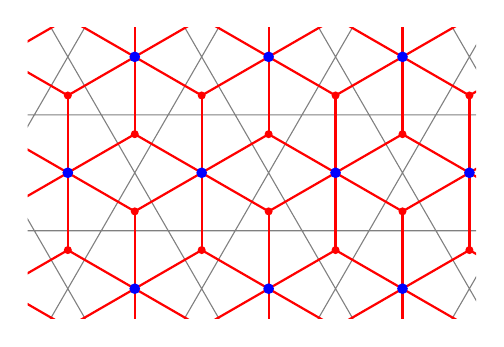
\begin{tikzpicture}[scale=0.85]
  \begin{scope}
  \clip (0.4,-0.45) rectangle (7.1,3.9);
  % kagome: corner-sharing triangles (medial graph of the triangular lattice of edge 2)
  \foreach \j in {-1,0,1,2} \foreach \i in {-2,-1,0,1,2,3} {
    \begin{scope}[shift={(2*\i+\j,1.732*\j)}]
      \draw[gray] (1,0) -- (1.5,0.866) -- (0.5,0.866) -- cycle;
      \draw[gray] (1.5,0.866) -- (2.5,0.866) -- (2,1.732) -- cycle;
    \end{scope}}
  % dual: hexagon centers (degree 6) are the vertices of the triangular lattice; triangle centers (degree 3)
  % are the centroids of its triangles
  \foreach \j in {-1,0,1,2} \foreach \i in {-2,-1,0,1,2,3} {
    \begin{scope}[shift={(2*\i+\j,1.732*\j)}]
      \draw[red,thick] (1,0.577) -- (0,0); \draw[red,thick] (1,0.577) -- (2,0); \draw[red,thick] (1,0.577) -- (1,1.732);
      \draw[red,thick] (2,1.155) -- (2,0); \draw[red,thick] (2,1.155) -- (1,1.732); \draw[red,thick] (2,1.155) -- (3,1.732);
      \fill[blue] (0,0) circle (0.08); \fill[red] (1,0.577) circle (0.06); \fill[red] (2,1.155) circle (0.06);
    \end{scope}}
  \end{scope}
\end{tikzpicture}
\diagramcaption{The kagom\'e lattice (gray) and its planar dual, the dice lattice (red). Blue vertices sit in the
hexagons and have degree 6; red vertices sit in the triangles and have degree 3.}\label{fig:dice}
\end{diagram}

$\Lambda^*$ is not an Archimedean lattice. In an Archimedean lattice every vertex is equivalent to every other, so all
vertices have the same degree, while $\Lambda^*$ has vertices of degree 3 and of degree 6. Its faces also fail the
other requirement: a rhombus with angles of $60^\circ$ and $120^\circ$ is not a regular polygon.

% ======================================================================
\subsection{Homework assignment 2}

\solution{2}{1}
At $T = 0$ the antiferromagnet ($J<0$, $K\to-\infty$, $v\to-1$) has $Z\to P(G,q)$, which counts the proper
$q$-colorings of $G$. These are the ground states, since no bond joins equal colors. The entropy per site at $T = 0$ is
therefore
\begin{equation}
  \bar S(T\to 0) = \kB\ln W,\qquad W(\Lambda,q) = \lim_{n\to\infty}P(G,q)^{1/n},
\end{equation}
where $G$ is a section of $\Lambda$ with $n$ vertices. The answer depends on $q$.

\solpart{$q = 3$.} Take $G$ to be a section of the triangular lattice made of triangles that share edges. In a proper
3-coloring the three vertices of every triangle carry all three colors. Once one triangle is colored, in $3! = 6$ ways,
each triangle sharing an edge with it has its third vertex forced to the remaining color, and this propagates through
the whole section. So $P(G,3) = 6$ for every $n$; these are the three-sublattice states of Figure~\ref{fig:tri3col}.
Then $W = \lim_{n\to\infty}6^{1/n} = 1$ and $\bar S\to 0$: the model obeys the Third Law for $q = 3$.

\solpart{$q\ge 4$.} The triangular lattice is tripartite, $\Lambda_{tri} = \Lambda_1\oplus\Lambda_2\oplus\Lambda_3$
(Figure~\ref{fig:kr}), and every neighbor of a site in $\Lambda_3$ lies in $\Lambda_1$ or $\Lambda_2$. Give every site
of $\Lambda_1$ color 1 and every site of $\Lambda_2$ color 2. Each site of $\Lambda_3$ can then take any of the $q-2$
other colors, independently of the others. This gives at least $(q-2)^{n/3}$ proper colorings, so
\begin{equation}
  W(tri,q)\ge(q-2)^{1/3}>1,\qquad \bar S(T\to 0)\ge\frac{\kB}{3}\ln(q-2)>0 .
\end{equation}
For $q\ge 4$ the ground-state entropy per site is nonzero and the Third Law fails. The bound grows with $q$, and so does
$W$. For $q = 4$ Baxter found $W(tri,4) = 1.4610$, above the bound $2^{1/3} = 1.2599$.

\solution{2}{2}
\solpart{(a)} Mean field theory gives $K_c = 1/\Delta$, i.e.\ $\kB T_c = J\Delta$ (Section~\ref{sec:mft}). On the strip
with $L_x$ vertices per row there are $e = 3L_x-2$ edges and $n = 2L_x$ vertices, so
$\Delta_{\text{eff}} = \lim_{L_x\to\infty}2e/n = 3$ and
\begin{equation}
  \kB T_{c,\text{MFT}} = 3J .
\end{equation}

\solpart{(b)} The actual critical temperature is $T_c = 0$. To prove it, build $Z$ from a transfer matrix that acts on
the two spins of a rung:
\begin{equation}
  T_{s,s'} = \exp\left[\frac{K}{2}(s_1s_2+s_1's_2')+K(s_1s_1'+s_2s_2')\right],
\end{equation}
a $4\times 4$ matrix. For $T>0$ all its entries are positive, so by the Perron--Frobenius theorem its largest
eigenvalue $\lambda_{\max}$ is nondegenerate. A simple root of the characteristic polynomial, whose coefficients are
analytic in $K$, is itself analytic in $K$, and $\lambda_{\max}>0$. So
$f = \lim_{n\to\infty}n^{-1}\ln Z = \frac{1}{2}\ln\lambda_{\max}$ is analytic for $0<T<\infty$, and there is no phase
transition at any finite temperature. At $T = 0$ the aligned states are the ground states and $\bar M_{sp} = \pm1$, so
the transition is at $T_c = 0$, as for the 1D chain. The Peierls argument of Lecture 11 shows the same thing: a domain
wall across the strip breaks two bonds, costing $\Delta U = 4J$, and can sit at about $L_x$ places, so
$\Delta G = 4J-\kB T\ln L_x<0$ for any $T>0$ once $L_x$ is large.

\solution{2}{3}
Call the pendant edge $e$. Deleting it leaves the square $C_4$ plus an isolated vertex; contracting it gives $C_4$.

\solpart{(a)} The deletion--contraction relation gives
\begin{equation}
  P(G,q) = P(G-e,q)-P(G/e,q) = qP(C_4,q)-P(C_4,q) = (q-1)P(C_4,q).
\end{equation}
With $P(C_n,q) = (q-1)^n+(-1)^n(q-1)$ from Lecture 9, $P(C_4,q) = (q-1)^4+(q-1) = q(q-1)(q^2-3q+3)$, so
\begin{equation}
  P(G,q) = q(q-1)^2(q^2-3q+3).
\end{equation}
For example $P(G,2) = 2$ and $P(G,3) = 36$.

\solpart{(b)} The same relation for $Z$ gives $Z(G,q,v) = qZ(C_4,q,v)+vZ(C_4,q,v) = (q+v)Z(C_4,q,v)$. For $C_4$, the
cluster formula sums over the $2^4$ edge subsets: a subset with $m<4$ edges has $4-m$ components, and the full square
has one. So
\begin{equation}
  Z(C_4,q,v) = \sum_{m=0}^{3}\binom4m q^{4-m}v^m+qv^4 = (q+v)^4+(q-1)v^4 ,
\end{equation}
the $n = 4$ case of $Z(C_n,q,v) = (q+v)^n+(q-1)v^n$ (Section~\ref{sec:pottszeros}). Therefore
\begin{equation}
  Z(G,q,v) = (q+v)\left[(q+v)^4+(q-1)v^4\right],
\end{equation}
which reduces to $P(G,q)$ at $v = -1$.

\solpart{(c)} Use $Z(G,q,v) = (x-1)^{k(G)}(y-1)^{n(G)}T(G,x,y)$ with $q = (x-1)(y-1)$, $v = y-1$, $k(G) = 1$ and
$n(G) = 5$. Then $q+v = x(y-1)$ and $q-1 = xy-x-y$, so
\begin{equation}
  Z(C_4,q,v) = (y-1)^4\left(x^4+xy-x-y\right) = (x-1)(y-1)^4\left(x^3+x^2+x+y\right),
\end{equation}
and $Z(G,q,v) = x(y-1)\,Z(C_4,q,v) = (x-1)(y-1)^5\,x\left(x^3+x^2+x+y\right)$. Hence
\begin{equation}
  T(G,x,y) = x^4+x^3+x^2+xy .
\end{equation}
This is $x\,T(C_4,x,y)$: a bridge multiplies the Tutte polynomial by $x$.

\solution{2}{4}
From $T(G,x,y) = x^4+x^3+x^2+xy$:
\begin{equation}
  N_{ST} = T(G,1,1) = 4,\qquad N_{SF} = T(G,2,1) = 30,\qquad N_{CSSG} = T(G,1,2) = 5 .
\end{equation}
Direct counts agree. A spanning tree must contain the pendant edge and three of the four edges of the square, which
gives 4. A spanning forest is any edge subset without a cycle; of the $2^5 = 32$ subsets only the two that contain the
whole square have one, which leaves 30. A connected spanning subgraph needs the pendant edge and at least three edges of
the square, which gives $4+1 = 5$.

\solution{2}{5}
The ladder has $n = 8$ vertices and $e = 4+2\cdot 3 = 10$ edges (four rungs, three edges along each leg). A spanning
subgraph is any subset of the edges together with all the vertices, so the number is
\begin{equation}
  N_{SSG} = 2^{e(G)} = 2^{10} = 1024 ,
\end{equation}
in agreement with $T(G,2,2) = 2^{e(G)}$.

\solution{2}{6}
Lecture 11 gives the mean-field self-consistency condition
$\bar M = I_1(K\Delta\bar M)/I_0(K\Delta\bar M)\simeq K\Delta\bar M/2$ for the $O(2)$ model, so
$K_{c,\text{MFT},O(2)} = 2/\Delta$ and $\kB T_{c,\text{MFT}} = J\Delta/2$. The hcp lattice has $\Delta = 12$
(Lecture 4), so
\begin{equation}
  \kB T_{c,\text{MFT}} = 6J .
\end{equation}

% ======================================================================
\subsection{Homework assignment 3}

\solution{3}{1}
The free energy is analytic in the high-temperature phase except where the argument of the logarithm can vanish. Let
$c = \cosh(2K)\ge 1$, so $\sinh^2(2K) = c^2-1$. Since $\mathcal P(\theta_1,\theta_2)\le 3$, with the maximum at
$\theta_1 = \theta_2 = 0$, the argument is bounded below:
\begin{equation}
  1+c^3-(c^2-1)\mathcal P\ \ge\ 1+c^3-3(c^2-1) = c^3-3c^2+4 = (c-2)^2(c+1)\ \ge\ 0 ,
\end{equation}
with equality only at $c = 2$ and $\theta_1 = \theta_2 = 0$. The singularity, and with it the critical point, is at
$\cosh(2K_c) = 2$:
\begin{equation}
  K_c = \frac{1}{2}\ln(2+\sqrt3) = 0.6585,\qquad \kB T_c = \frac{2J}{\ln(2+\sqrt3)} = 1.519\,J .
\end{equation}
Equivalently $\tanh K_c = [(c-1)/(c+1)]^{1/2} = 1/\sqrt3$. The lattice is the honeycomb lattice, with coordination
number 3.

\solution{3}{2}
Yes: $a = 1$ and $b = 0$. The correlation function is continuous in $T$, and at $T_c$ both moduli equal 1. From below,
$\ev{\sigma_{(0,0)}\sigma_{(1,1)}}\to(2/\pi)E(1) = 2/\pi$. From above, $E(k_>)\to 1$ while
$K(k_>)\simeq\ln\left[4/(1-k_>^2)^{1/2}\right]$ diverges and $(k_>^2-1)K(k_>)\to 0$. The high-temperature expression
stays finite at $T_c$ only if $b = 0$, and continuity then requires $a = 1$:
\begin{equation}
  \ev{\sigma_{(0,0)}\sigma_{(1,1)}} = \frac{2}{\pi}\left[E(k_>)+(k_>^2-1)K(k_>)\right],\qquad T>T_c .
\end{equation}
The limit $T\to\infty$ gives a check. There $k_>\to 0$ and $E(0) = K(0) = \pi/2$, so the form tends to $a+b-1$, which
must vanish because the spins become independent. It does.

Remark: the form given in the problem lacks an overall factor $1/k_>$. Two paths of length 2 join $(0,0)$ and
$(1,1)$, so the high-temperature expansion starts with $2v^2\simeq 2K^2$. The expression above starts with
$k_>^2/2\simeq 8K^4$, and the same expression divided by $k_>$ starts with $k_>/2\simeq 2K^2$. A transfer-matrix
calculation on an infinitely long cylinder of circumference 12 at $K = 0.3$ gives 0.2073, against 0.2071 with the factor
$1/k_>$ and 0.0839 without it. Both expressions equal $2/\pi$ at $T_c$, where $k_> = 1$, so the answer to
Problem~3.5 is unaffected.

\solution{3}{3}
\solpart{(a)} $f(\lambda^ax,\lambda^by) = \lambda^{ap+bq}f(x,y)$, so $f$ is a generalized homogeneous function exactly
when $ap+bq = 1$. This holds for a one-parameter family: any $a\ne 0,1/p$ with $b = (1-ap)/q$, for example
$a = 1/(2p)$, $b = 1/(2q)$.

\solpart{(b)} Both terms must scale with $\lambda^1$: $ap+bq = 1$ and $ar+bs = 1$. Since $ps\ne qr$ the solution is
unique,
\begin{equation}
  a = \frac{s-q}{ps-qr},\qquad b = \frac{p-r}{ps-qr},
\end{equation}
and both are nonzero because $q\ne s$ and $p\ne r$. So $f$ is a generalized homogeneous function with these exponents.

\solpart{(c)} Not for generic coefficients. Fix $x$ and $y$, write $C = c_2x^py^q$, $D = c_4x^ry^s$,
$\alpha = ap+bq$ and $\beta = ar+bs$, and suppose that
\begin{equation}
  g(\lambda)\equiv\frac{c_1+C\lambda^\alpha}{c_3+D\lambda^\beta} = \lambda\,g(1)\qquad\text{for all }\lambda>0 .
\end{equation}
As $\lambda\to 0$ the left side behaves as $\lambda^{\min(\alpha,0)-\min(\beta,0)}$ times a nonzero constant, and the
right side vanishes linearly. If $\alpha<0$ this needs $\beta<0$ with $\alpha-\beta = 1$; then as $\lambda\to\infty$ the
left side tends to the constant $c_1/c_3$ while the right side grows, a contradiction. So $\alpha\ge 0$ and
$\beta = -1$. As $\lambda\to\infty$ the left side then grows as $(C/c_3)\lambda^\alpha$, which needs $\alpha = 1$. With
$\alpha = 1$ and $\beta = -1$ the condition reads $(c_1+C\lambda)(c_3+D) = (c_1+C)(c_3\lambda+D)$ for all $\lambda$, and
comparing coefficients gives $CD = c_1c_3$. But $CD = c_2c_4x^{p+r}y^{q+s}$ changes with $x$ and $y$, since $p+r$ and
$q+s$ are generic, so it cannot equal the constant $c_1c_3$ everywhere. Hence $f$ is not a generalized homogeneous
function.

\solpart{(d)} $f(\lambda^ax,\lambda^by) = \lambda^ax\tanh(\lambda^{2b}y^2)$ would have to equal $\lambda x\tanh(y^2)$ for
all $x$, $y$. Letting $y\to\infty$ at fixed $\lambda$ gives $\lambda^a = \lambda$, so $a = 1$; then
$\tanh(\lambda^{2b}y^2) = \tanh(y^2)$ for all $y$ forces $b = 0$, which is excluded. So $f$ is not a generalized
homogeneous function.

\solution{3}{4}
\solpart{(a)} The relations of Section~\ref{sec:exprel} give
\begin{gather}
  \alpha = 2-2\beta-\gamma = 2-\frac{2}{3}-\frac{5}{4} = \frac{1}{12}\quad\text{(Rushbrooke)},\\
  \delta = 1+\frac{\gamma}{\beta} = 1+\frac{15}{4} = \frac{19}{4}\quad\text{from }\gamma = \beta(\delta-1),\\
  \nu = \frac{2-\alpha}{d} = \frac{23}{12d}\quad\text{(hyperscaling)},\qquad
  \eta = 2-\frac{\gamma}{\nu} = 2-\frac{15d}{23}\quad\text{from }\gamma = \nu(2-\eta).
\end{gather}
The problem leaves $d$ open, and $\nu$ and $\eta$ depend on it through hyperscaling. For $d = 3$, $\nu = 23/36 = 0.639$
and $\eta = 1/23 = 0.043$. Together with $\beta = 1/3$ and $\gamma = 5/4$ these are close to the 3D Ising values, which
points to a three-dimensional substance.

\solpart{(b)} From Section~\ref{sec:exprel}, $a_\tau = 1/[\beta(\delta+1)] = 12/23$ and $a_h = \delta/(\delta+1) = 19/23$,
so
\begin{equation}
  y_\tau = a_\tau d = \frac{12d}{23},\qquad y_h = a_hd = \frac{19d}{23}.
\end{equation}
These satisfy $y_\tau = 1/\nu$ and $y_h = (d+2-\eta)/2$. For $d = 3$, $y_\tau = 36/23 = 1.565$ and
$y_h = 57/23 = 2.478$.

\solution{3}{5}
At $T = T_c$, $k = 1$ and $E(1) = 1$. $K(k)$ diverges only logarithmically, so $(k^2-1)K(k)\to 0$ and
$(k^2-1)^2K(k)^2\to 0$. Then
\begin{equation}
  \ev{\sigma_{(0,0)}\sigma_{(2,2)}}_{T_c} = \frac{4}{3\pi^2}(5-1) = \frac{16}{3\pi^2} = 0.5404 .
\end{equation}
With $\ev{\sigma_{(0,0)}\sigma_{(1,1)}}_{T_c} = 2/\pi = 0.6366$ from Problem~3.2, the ratio is
\begin{equation}
  \frac{\ev{\sigma_{(0,0)}\sigma_{(2,2)}}}{\ev{\sigma_{(0,0)}\sigma_{(1,1)}}}\bigg|_{T_c} = \frac{8}{3\pi} = 0.8488 .
\end{equation}
The two spins are at distances $\sqrt2$ and $2\sqrt2$, so in $d = 2$ with $\eta = 1/4$ the scaling form predicts
$(2\sqrt2/\sqrt2)^{-1/4} = 2^{-1/4} = 0.8409$. The exact ratio is within 1\% of the prediction, although the distances
are only one or two lattice spacings along the diagonal.

% ======================================================================
\subsection{Homework assignment 4}

\solution{4}{1}
The linearized RG matrix is
\begin{equation}
  M = \begin{pmatrix}\pder{z'}{z} & \pder{z'}{y}\\[6pt] \pder{y'}{z} & \pder{y'}{y}\end{pmatrix}
  = \begin{pmatrix}\dfrac{8z(1-z^2)}{(1+z^2)^3} & 0\\[10pt] \dfrac{-4zy^4}{(1+z^2)^3} & \dfrac{4y^3}{(1+z^2)^2}\end{pmatrix}.
\end{equation}
It is lower triangular, so its eigenvalues are the diagonal elements, and in the notation of Lecture 17,
$\hat{\mathbf e}_2 = (0,1)$ and $\hat{\mathbf e}_1\propto\left(a^{-1}(\lambda_1-\lambda_2),1\right)$ with $a = M_{21}$.
At the fixed point $z_*$ solves $(1+z^2)^2 = 4z$, i.e.\ $(z-1)(z^3+z^2+3z-1) = 0$, so $z_* = 0.295598$ is the real root
of the cubic, and $y_*^3 = (1+z_*^2)^2$ gives $y_* = 1.057435$. These identities simplify the entries.

\solpart{(i)} $\lambda_1 = 8z_*(1-z_*^2)/(1+z_*^2)^3 = 2(1-z_*^2)/(1+z_*^2) = 1.6786$.

\solpart{(ii)} With $b = 2$, $y_1 = \ln\lambda_1/\ln 2 = 0.7472$.

\solpart{(iii)} $a = -4z_*y_*^4/(1+z_*^2)^3 = -4z_*y_*/(1+z_*^2) = -1.1498$, so
$a^{-1}(\lambda_1-\lambda_2) = (1.6786-4)/(-1.1498) = 2.0189$ and
\begin{equation}
  \hat{\mathbf e}_1 = \frac{(2.0189,\,1)}{\left(2.0189^2+1\right)^{1/2}} = (0.8961,\,0.4439),\qquad
  \theta_1 = 26.35^\circ .
\end{equation}

\solpart{(iv)} $\lambda_2 = 4y_*^3/(1+z_*^2)^2 = 4$ exactly. (The rounded values quoted in the problem give 3.995.)

\solpart{(v)} $y_2 = \ln 4/\ln 2 = 2$.

\solpart{(vi)} $\hat{\mathbf e}_2 = (0,1)$, $\theta_2 = 90^\circ$.

Both eigenvalues exceed 1, so this fixed point repels along both eigenvectors; it is the red point of
Figure~\ref{fig:spin1flow}. Since $\lambda_2>\lambda_1$, the flow leaves it tangent to $\hat{\mathbf e}_1$ and then
turns toward the vertical.

\solution{4}{2}
Write $e^{K\sigma\sigma'} = \cosh K\,(1+v\sigma\sigma')$. Summing over the spins leaves the closed subgraphs:
\begin{equation}
  Z = 2^N(\cosh K)^{N_b}\sum_{\text{closed }G'}v^{e(G')},
\end{equation}
where $N_b = \Delta N/2 = 3N$ is the number of bonds of the triangular lattice ($\Delta = 6$). The smallest closed
subgraphs are the elementary triangles. Each site lies on six of them and each has three sites, so there are $2N$, and
$Z = 2^N(\cosh K)^{3N}\left[1+2Nv^3+\Order(v^4)\right]$. Then
\begin{equation}
  f = \ln 2+3\ln\cosh K+2v^3+\ldots,
\end{equation}
so $a = 3$, $b = 2$, $p = 3$.

\solution{4}{3}
From Lecture 7, $\beta^{-1}\bar\chi = \sum_{\mathbf r}\ev{\sigma_0\sigma_{\mathbf r}}$. In the high-temperature
expansion $\ev{\sigma_0\sigma_{\mathbf r}}$ starts at order $v^{\ell}$, where $\ell$ is the length of the shortest path
from 0 to $\mathbf r$. To order $v$ only $\mathbf r = 0$ (which gives 1) and the $\Delta = 6$ nearest neighbors (which
give $v$ each) contribute:
\begin{equation}
  \bar\chi = \beta\left[1+6v+\Order(v^2)\right],
\end{equation}
so the $\Order(v)$ term is $6\beta v$.

\solution{4}{4}
To first order in $K$,
\begin{equation}
  \ev{\mathbf S_0\cdot\mathbf S_1} = \frac{\ev{\cos(\theta_0-\theta_1)\left[1+K\sum_{e}\cos(\theta_{\mathbf r}-\theta_{\mathbf r'})\right]}_0}
  {\ev{1+K\sum_{e}\cos(\theta_{\mathbf r}-\theta_{\mathbf r'})}_0}
  = K\ev{\cos^2(\theta_0-\theta_1)}_0 = \frac{K}{2},
\end{equation}
where $\ev{\cdots}_0$ is the average over independent angles. Only the bond joining the two spins contributes. In terms
of the character expansion $e^{K\cos\phi} = I_0(K)\left[1+2\sum_{n\ge1}t_n\cos n\phi\right]$ with
$t_n = I_n(K)/I_0(K)$, the leading term is $t_1 = I_1(K)/I_0(K) = K/2+\Order(K^3)$. The lattice, here the
four-dimensional hypercubic one, first enters at order $t_1^3$, through the plaquettes that contain the bond.

\solution{4}{5}
At $T = 0$ the ground states are all spins up or all down, with every one of the $N_b = dN$ bonds satisfied. The
lowest excitation reverses one spin, which breaks its $2d$ bonds; each broken bond changes $K\sigma\sigma'$ from $K$ to
$-K$, so the weight is $e^{-2K\cdot 2d} = z^{2d}$, and there are $N$ choices. So
$Z = 2e^{dNK}\left[1+Nz^{2d}+\ldots\right]$, and
\begin{equation}
  f = dK+z^{2d}+\ldots ,
\end{equation}
so $a = d$, $b = 1$, $p = 2d$. (Two adjacent reversed spins break $2(2d-1)$ bonds and enter at order $z^{4d-2}$.)

% ======================================================================
\subsection{Homework assignment 5}

\solution{5}{1}
The first coefficient is $12 = \Delta$, and the lattice is the fcc lattice.

\solpart{(a)} If $\tilde\chi\sim A(1-v/v_c)^{-\gamma}$, the coefficients satisfy
$a_n/a_{n-1}\simeq v_c^{-1}\left[1+(\gamma-1)/n\right]$, so $a_{n-1}/a_n$ estimates $v_c$:
\begin{center}
\small
\renewcommand{\arraystretch}{1.15}
\begin{tabular}{rccc}
  $n$ & $a_n/a_{n-1}$ & $v_c$ & $K_c$\\ \hline
  2 & 11.000000 & 0.090909 & 0.091161\\
  3 & 10.636364 & 0.094017 & 0.094296\\
  4 & 10.435897 & 0.095823 & 0.096118\\
  5 & 10.313677 & 0.096959 & 0.097264\\
  6 & 10.232748 & 0.097725 & 0.098038\\
  7 & 10.175344 & 0.098277 & 0.098595\\
  8 & 10.132256 & 0.098695 & 0.099017\\
  9 & 10.098679 & 0.099023 & 0.099348\\
  10 & 10.071789 & 0.099287 & 0.099615\\
  11 & 10.049784 & 0.099505 & 0.099835
\end{tabular}
\end{center}
with $K_c = \operatorname{arctanh}v_c$. The estimates increase steadily because of the $1/n$ correction. Extrapolating
the last two ratios linearly in $1/n$ gives $11r_{11}-10r_{10} = 9.8297$, so $v_c\simeq 0.10173$, and the slope gives
$\gamma\simeq 1.246$.

\solpart{(b)} Let $D(v) = \dd\ln\tilde\chi/\dd v$. From the series,
\begin{equation}
  D(v) = 12+120v+1188v^2+11664v^3+114492v^4+1124856v^5+11057268v^6+\ldots ,
\end{equation}
and the $[3,3]$ Pad\'e approximant $P_3(v)/Q_3(v)$ that matches these seven terms is
\begin{gather}
  P_3(v) = 12-62.5937v+142.4784v^2-35.8271v^3,\\
  Q_3(v) = 1-15.2161v+65.0346v^2-118.9337v^3 .
\end{gather}
Near $v_c$, $\tilde\chi\sim(1-v/v_c)^{-\gamma}$ gives $D\simeq-\gamma/(v-v_c)$: a simple pole with residue $-\gamma$.
$Q_3$ has one real root, $v = 0.10171$, and a complex pair $0.2226\pm 0.1820\,\ii$ farther from the origin. The real
root gives
\begin{equation}
  v_c = 0.10171,\qquad K_c = \operatorname{arctanh}v_c = 0.10206,\qquad
  \gamma = -\frac{P_3(v_c)}{Q_3'(v_c)} = 1.245 .
\end{equation}
The accepted values for the fcc lattice are $K_c = 0.10207$ and $\gamma = 1.237$.

\solution{5}{2}
The critical temperature is $\kB T_c = 8a/(27b)$, and $a/(4b) = (27/32)\kB T_c = 0.84\,\kB T_c$: this isotherm lies
below $T_c$ and has a van der Waals loop. Part of it is mechanically unstable, with $\partial p/\partial v>0$ and hence
$\kappa_T<0$:
\begin{equation}
  \pder{p}{v} = -\frac{\kB T}{(v-b)^2}+\frac{2a}{v^3}>0\iff 8b(v-b)^2>v^3 .
\end{equation}
With $x = v/b$ this is $x^3-8x^2+16x-8 = (x-2)(x^2-6x+4)<0$. The roots are $x = 2$ and $x = 3\pm\sqrt5$; the root
$3-\sqrt5 = 0.76$ lies in the excluded region $v<b$. So the isotherm is unphysical for
\begin{equation}
  2b<v<(3+\sqrt5)\,b = 5.236\,b .
\end{equation}
At $v = 2b$ the isotherm has its local minimum, where it just touches $p = 0$; at $v = (3+\sqrt5)b$ it has its local
maximum, $p = (5\sqrt5-11)a/(8b^2) = 0.0225\,a/b^2$. In equilibrium the Maxwell construction replaces the loop by the
coexistence line $p = 0.0181\,a/b^2$, which runs from $v_\ell = 1.645\,b$ to $v_g = 9.72\,b$. Between $v_\ell$ and $2b$,
and between $5.236\,b$ and $v_g$, the vdW curve describes metastable superheated liquid and supercooled gas. Values
$v\le b$ are excluded altogether.

\solution{5}{3}
This is the Peng--Robinson form of the equation of state, with a temperature-independent $a$. Use $x = v/b$,
$t = \kB Tb/a$, $\pi = pb^2/a$ and $g(x) = x^2+2x-1$, so that $\pi = t/(x-1)-1/g$. The critical point has
\begin{equation}
  \pder{\pi}{x} = 0:\ \frac{t}{(x-1)^2} = \frac{2(x+1)}{g^2},\qquad
  \frac{\partial^2\pi}{\partial x^2} = 0:\ \frac{2t}{(x-1)^3} = \frac{6x^2+12x+10}{g^3}.
\end{equation}
Dividing the second by the first gives $4(x+1)g = (x-1)(6x^2+12x+10)$, i.e.
\begin{equation}
  x^3-3x^2-3x-3 = 0 .
\end{equation}
With $x = 1+w$ this becomes $w^3-6w-8 = 0$, and Cardano's formula gives its real root,
$w = (4+2\sqrt2)^{1/3}+(4-2\sqrt2)^{1/3}$.

\solpart{(a)} $v_c = \left[1+(4+2\sqrt2)^{1/3}+(4-2\sqrt2)^{1/3}\right]b = 3.9514\,b$.

\solpart{(b)} $t_c = 2(x_c+1)(x_c-1)^2/g(x_c)^2 = 0.17014$, so $\kB T_c = 0.1701\,a/b$.

\solpart{(c)} $\pi_c = t_c/(x_c-1)-1/g(x_c) = 0.013237$, so $p_c = 0.01324\,a/b^2$.

\solpart{(d)} $z_c = p_cv_c/(\kB T_c) = \pi_cx_c/t_c = 0.3074$. The measured values in Lecture 23 are 0.288 to 0.294
for Xe, Ar, N$_2$, O$_2$, CO and CH$_4$, and 0.304 and 0.308 for H$_2$ and He; H$_2$O (0.230) and CO$_2$ (0.275) are
lower. This equation of state comes within about 0.015 of the simple gases. Van der Waals gives $3/8 = 0.375$, and
Dieterici gives $2/e^2 = 0.271$.

\solpart{(e)} Expand in $\rho = 1/v$:
\begin{equation}
  \frac{1}{v-b} = \rho+b\rho^2+b^2\rho^3+\ldots,\qquad
  \frac{1}{v^2+2bv-b^2} = \rho^2-2b\rho^3+\ldots ,
\end{equation}
so $p/(\kB T) = \rho+B_2\rho^2+B_3\rho^3+\ldots$ with
\begin{equation}
  B_2 = b-\frac{a}{\kB T},\qquad B_3 = b^2+\frac{2ab}{\kB T}.
\end{equation}
$B_2$ is the same as for van der Waals, so the Boyle temperature is again $\kB T_{\text{Boyle}} = a/b$; $B_3$ picks up
the extra term $2ab/(\kB T)$. (The photograph of the handout ends at this point, so any further part of the question
is not available.)
